\documentclass[aspectratio=169]{beamer}

% Theme. Madrid is built into beamer (no extra packages needed). Swap for
% metropolis etc. if installed.
\usetheme{Madrid}
\usecolortheme{default}
\setbeamertemplate{navigation symbols}{}   % drop nav clutter
\setbeamertemplate{caption}[numbered]

\usepackage[T1]{fontenc}
\usepackage[utf8]{inputenc}
\usepackage{graphicx}
\usepackage{booktabs}
\usepackage{amsmath,amssymb}

% Figures live in the repo-level results/ directory; reference them in place
% via bare filenames (e.g. acc_vs_noise.png) rather than copying into slides/.
\graphicspath{{../results/}}

\title[SVA Robustness to Noise]{Does Syntactic Structure Make Language Models\\
       More Robust to Noise?}
\subtitle{LSTM vs.\ RNNG Subject--Verb Agreement Under Training-Data Corruption}
\author[Wilke, Fu, Garimella]{Jackson Wilke \and Kelly Fu \and Sanjana Garimella}
\institute[UCSD]{DSC 291: Language Models as Cognitive Models \\ UC San Diego}
\date{June 2026}

\begin{document}

\begin{frame}[plain]
  \titlepage
\end{frame}

\begin{frame}{Outline}
  \tableofcontents
\end{frame}

\section{Motivation}

% OWNER: Kelly Fu (intro per proposal)

\begin{frame}{Motivation: Can grammar survive noisy input?}
  % TODO (Kelly): children acquire robust SVA despite noisy input (speech
  % errors, non-native speech, agreement violations).
  % TODO (Kelly): poverty-of-the-stimulus framing -> how robust are LMs?
\begin{itemize}
\item Children acquire robust grammatical systems despite hearing noisy and imperfect language
\item This observation motivates the classic \textbf{Poverty of the Stimulus} debate:

      Is grammar learned from data, or supported by innate structure?
\item Human experiments cannot systematically manipulate children's linguistic input
\item Neural language models provide a controllable testbed:
\begin{itemize}
\item architecture = innate structure
\item training corpus = linguistic environment
\end{itemize}

\end{itemize}

\end{frame}


\begin{frame}{Research Questions}

\textbf{RQ1: Can grammar be learned from noisy input?}

\begin{itemize}
    \item How much grammatical corruption can a model tolerate?
    \item Is there a critical noise threshold beyond which acquisition breaks down?
\end{itemize}


\textbf{RQ2: How does noise change generalization?}

\begin{itemize}
    \item Does the model maintain a hierarchical syntactic rule?
    \item Or does it fall back on a simpler linear nearest-noun heuristic?
\end{itemize}


\textbf{RQ3: Does structure buy robustness?}

\begin{itemize}
    \item Compare LSTM and RNNG under identical noise conditions.
    \item Does explicit syntactic bias help preserve grammatical learning?
\end{itemize}

\end{frame}

\section{Background}

% OWNER: Kelly Fu (background per proposal)

\begin{frame}{Subject--verb agreement: hierarchical vs.\ linear & Attractors as the diagnostic case}
  % I combined 2 parts together since they are both talking about hierarchical vs.\ linear.
  % TODO (Kelly): hierarchical rule (agree with true subject) vs. linear
  % heuristic (agree with nearest noun); attractor example
  % "the keys to the cabinet are/is...".
  \begin{itemize}
  %  \item TODO


  \end{itemize}
\end{frame}

\begin{frame}{Attractors as the diagnostic case}
  % TODO (Kelly): why the attractor gap dissociates the two rules; minimal
  % pair evaluation paradigm (BLiMP / SyntaxGym lineage).
  \begin{itemize}
    \item TODO
%  \end{itemize}
%\end{frame}

\begin{frame}{Architectural inductive biases: LSTM and RNNG}
  
  \begin{itemize}
   
  \end{itemize}
\end{frame}


\begin{frame}{Prior work}
  % TODO (Kelly): Linzen 2016, Gulordava 2018 (LSTMs), Dyer 2016 / Kuncoro
  % 2018 (RNNG structural bias). Gap: behavior under *noisy* supervision.
  \begin{itemize}
   % \item TODO
    
  \end{itemize}
\end{frame}

\section{Methods}

% OWNER: Jackson Wilke (methods/setup per proposal)

\begin{frame}{Noise injection: five corrupted corpora}
  % TODO (Jackson): flip SVA with prob p in {0.0, 0.004, 0.02, 0.10, 0.50};
  % all other properties preserved; training-set size held constant.
  \begin{itemize}
    \item TODO
  \end{itemize}
\end{frame}

\begin{frame}{Leak-free evaluation protocol}
  % TODO (Jackson): fixed 20k held-out indices (seed 1234) excluded from every
  % training corpus; minimal pairs built from the *clean* version of those rows.
  \begin{itemize}
    \item TODO
  \end{itemize}
\end{frame}

\begin{frame}{Models and metrics}
  % TODO (Jackson): LSTM (Gulordava-style) vs. RNNG (aistairc/rnng-pytorch);
  % metrics: minimal-pair accuracy, attractor gap, target-verb surprisal;
  % seeds {1,2,3}.
  \begin{itemize}
    \item TODO
  \end{itemize}
\end{frame}

\section{Results}

\begin{frame}{Accuracy holds up until 50\% noise}
  \begin{columns}[T]
    \begin{column}{0.55\textwidth}
      \centering
      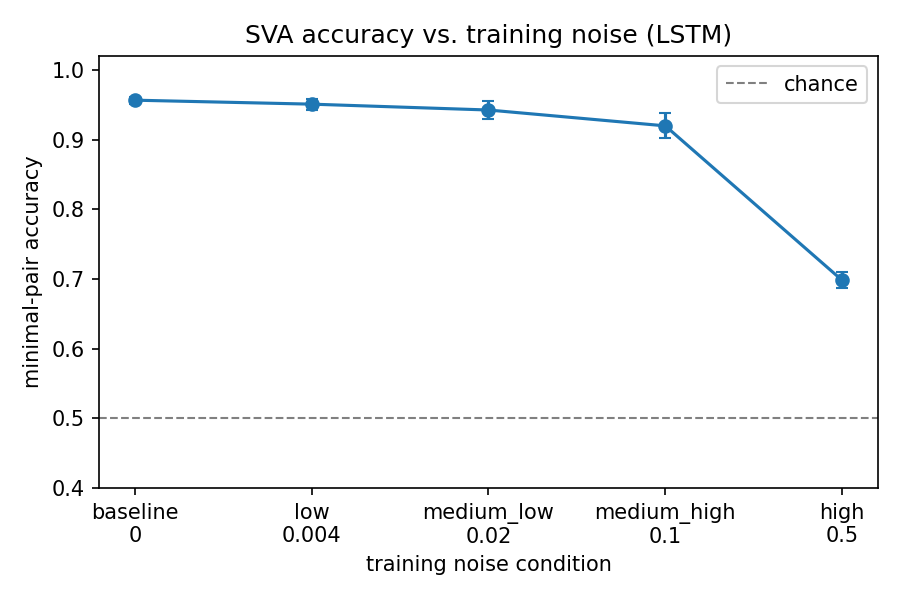
\includegraphics[width=\linewidth,height=0.65\textheight,keepaspectratio]{acc_vs_noise.png}
    \end{column}
    \begin{column}{0.45\textwidth}
      \small
      \begin{itemize}
        \item Stays flat up to $10\%$ noise ($0.961 \to 0.934$)
        \item Drops sharply at $50\%$, down to $0.708$
        \item The model can handle about 1 bad verb in 10 before it breaks
        \item Not a gradual decline, more like a threshold
      \end{itemize}
    \end{column}
  \end{columns}
\end{frame}

\begin{frame}{The attractor gap grows with noise}
  \begin{columns}[T]
    \begin{column}{0.55\textwidth}
      \centering
      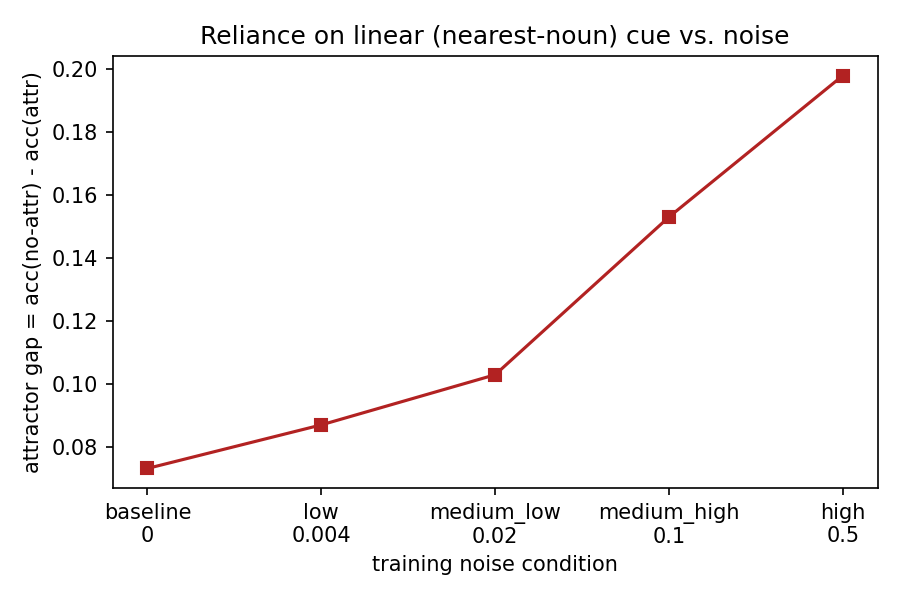
\includegraphics[width=\linewidth,height=0.65\textheight,keepaspectratio]{attractor_gap.png}
    \end{column}
    \begin{column}{0.45\textwidth}
      \small
      \begin{itemize}
        \item Gap $=$ acc(no attractor) $-$ acc(attractor)
        \item Goes from $0.073$ to $0.198$ as noise increases
        \item Tells us how much the model leans on the nearest-noun shortcut
        \item More noise means more reliance on the linear rule
      \end{itemize}
    \end{column}
  \end{columns}
\end{frame}

\begin{frame}{Attractor items are where it falls apart}
  \begin{columns}[T]
    \begin{column}{0.55\textwidth}
      \centering
      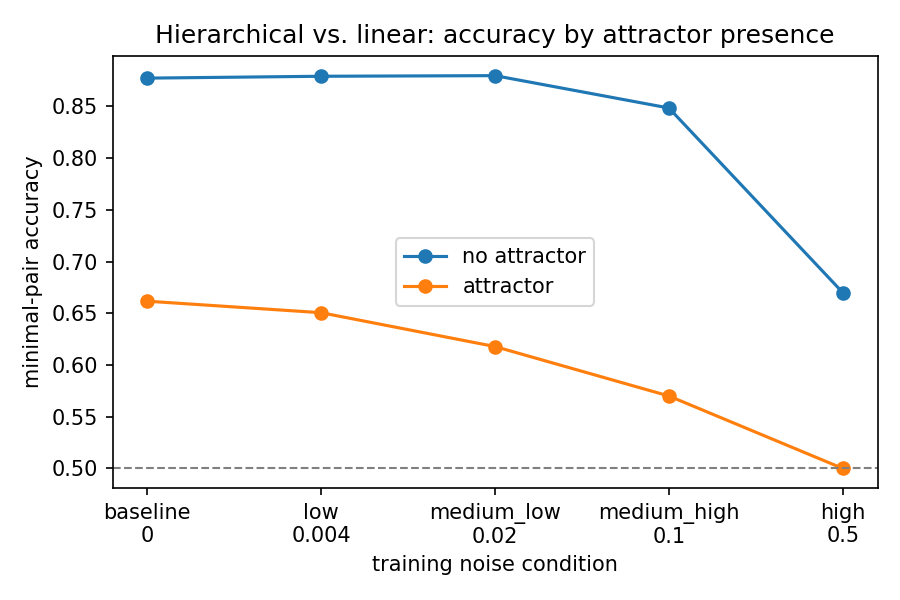
\includegraphics[width=\linewidth,height=0.65\textheight,keepaspectratio]{acc_by_attractor.png}
    \end{column}
    \begin{column}{0.45\textwidth}
      \small
      \begin{itemize}
        \item Without attractors, accuracy stays above $0.94$ until $50\%$
        \item With attractors, it drops to near chance ($0.525$)
        \item Attractor items are the only cases where the two rules disagree
        \item So that's exactly where the model struggles first
      \end{itemize}
    \end{column}
  \end{columns}
\end{frame}

\begin{frame}{Learning over time: delay vs.\ prevention}
  \begin{columns}[T]
    \begin{column}{0.55\textwidth}
      \centering
      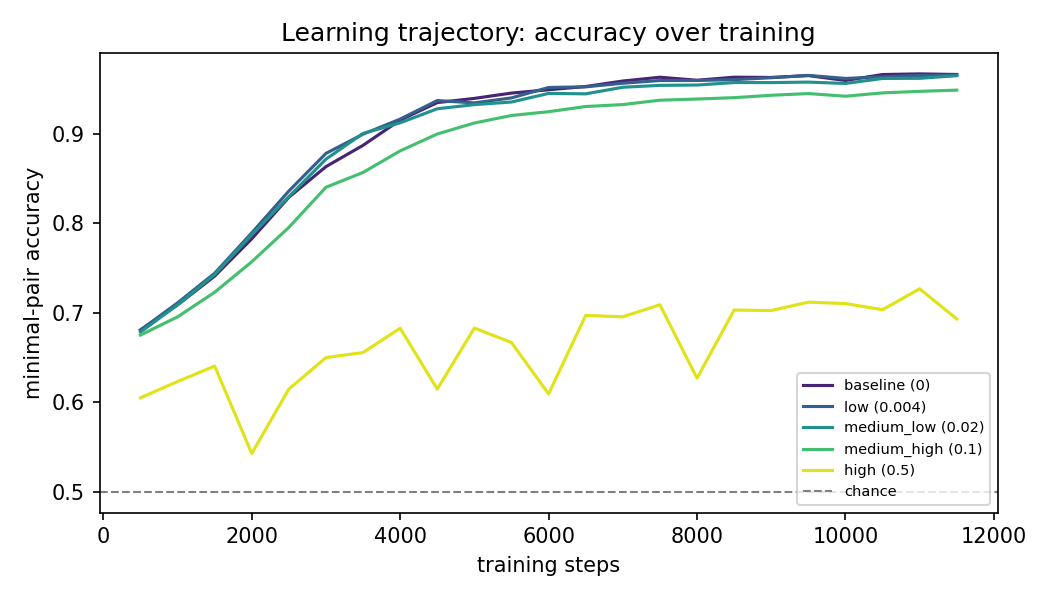
\includegraphics[width=\linewidth,height=0.65\textheight,keepaspectratio]{acc_trajectory.png}
    \end{column}
    \begin{column}{0.45\textwidth}
      \small
      \begin{itemize}
        \item Up to $10\%$ noise: reaches the same accuracy, just takes longer (\textbf{delay})
        \item At $50\%$: plateaus around $0.69$ and never catches up (\textbf{prevention})
        \item Clean model: gap shrinks over training ($0.15 \to 0.05$)
        \item $50\%$ model: gap actually \emph{grows} ($0.14 \to 0.20$)
      \end{itemize}
    \end{column}
  \end{columns}
\end{frame}

\begin{frame}{Does structure help? RNNG vs.\ LSTM}
  \begin{columns}[T]
    \begin{column}{0.55\textwidth}
      \centering
      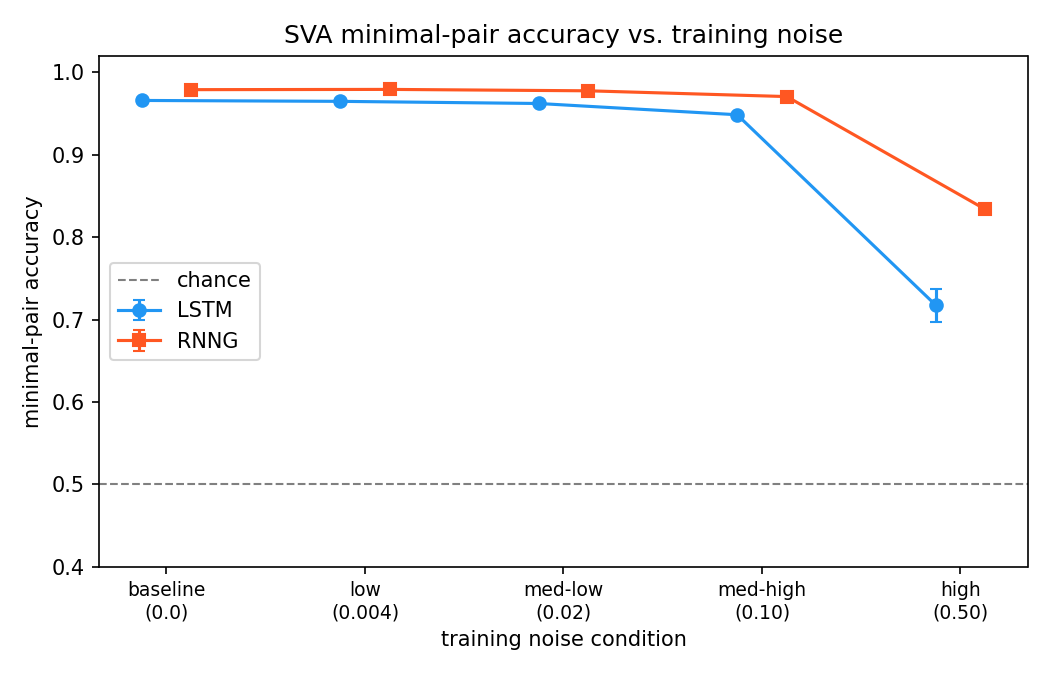
\includegraphics[width=\linewidth,height=0.65\textheight,keepaspectratio]{combined_acc_vs_noise.png}
    \end{column}
    \begin{column}{0.45\textwidth}
      \small
      \begin{itemize}
        \item RNNG $=$ LSTM plus an explicit syntactic (tree) bias
        \item More accurate than the LSTM at \emph{every} noise level
        \item Gap widens where noise bites hardest: at $50\%$, $0.834$ vs.\ $0.708$
        \item Same held-out set ($\sim$20k pairs); single full-scale seed so far
      \end{itemize}
    \end{column}
  \end{columns}
\end{frame}

\begin{frame}{RNNG keeps the hierarchical rule under noise}
  \begin{columns}[T]
    \begin{column}{0.55\textwidth}
      \centering
      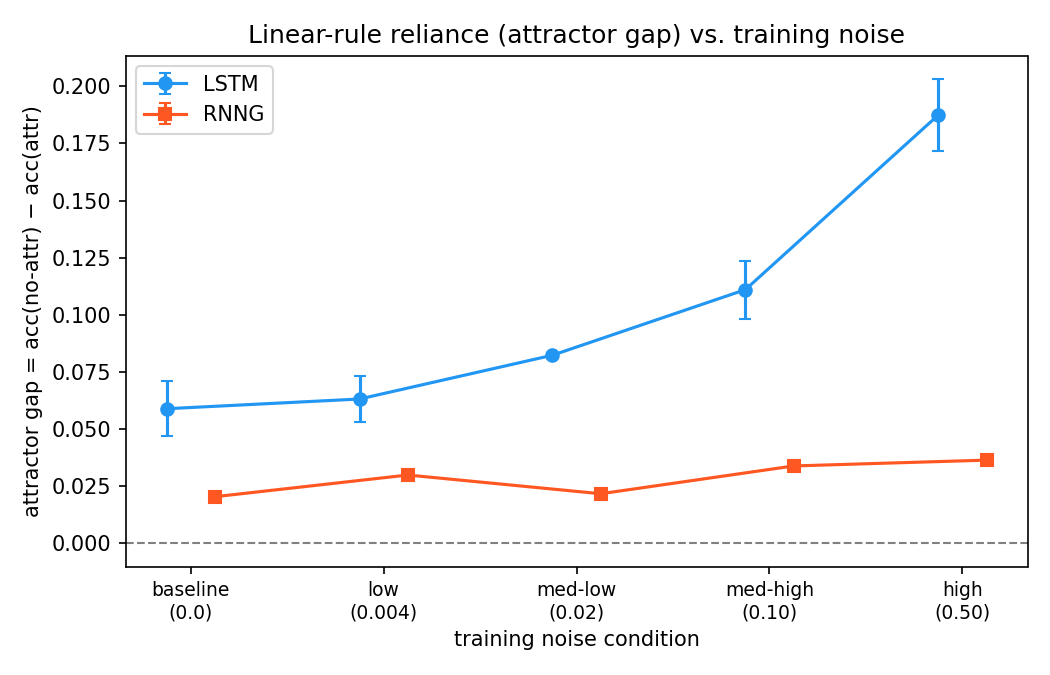
\includegraphics[width=\linewidth,height=0.65\textheight,keepaspectratio]{combined_attractor_gap.png}
    \end{column}
    \begin{column}{0.45\textwidth}
      \small
      \begin{itemize}
        \item LSTM's attractor gap grows $2.7\times$ with noise ($0.073 \to 0.198$)
        \item RNNG's stays low and flat ($0.020 \to 0.036$)
        \item At $50\%$ noise the RNNG gap is \emph{half} the LSTM's clean-data gap
        \item Structural bias preserves the hierarchical rule where the LSTM defaults to the linear shortcut
      \end{itemize}
    \end{column}
  \end{columns}
\end{frame}

\section{Discussion}

% OWNER: Sanjana Garimella (discussion per proposal)

\begin{frame}{When does the rule break?}
  \begin{itemize}
    \item \textbf{Threshold, not gradual}: absorbs noise up to $10\%$, snaps at $50\%$
      --- like a child's grammar surviving occasional speech errors.
    \item \textbf{Attractor gap is the early warning}: it climbs ($0.07 \to 0.20$)
      while overall accuracy still looks healthy.
    \item \textbf{Delay vs.\ prevention}: low noise only \emph{delays} acquisition
      (curves converge); $50\%$ noise \emph{prevents} it and entrenches the linear rule.
  \end{itemize}
\end{frame}

\begin{frame}{Does structure buy robustness?}
  \begin{itemize}
    \item The headline question --- does a syntactic prior (RNNG) resist noise
      better than a sequential LSTM? --- needs the RNNG runs (in progress).
    \item \textbf{LSTM baseline}: no explicit hierarchy bias $\Rightarrow$ learns the
      rule cleanly when input is clean, but drifts to the linear shortcut as noise grows.
    \item If RNNG holds the hierarchical rule where the LSTM has caved
      $\Rightarrow$ structure buys robustness.
    \item If both fail together $\Rightarrow$ the bottleneck is input quality, not
      architecture --- speaking to poverty-of-the-stimulus.
  \end{itemize}
\end{frame}

\begin{frame}{Takeaways and future work}
  \textbf{Takeaways}
  \begin{itemize}
    \item LSTMs tolerate moderate SVA noise but have a sharp breaking point.
    \item Noise trades the hierarchical rule for the linear nearest-noun heuristic.
    \item Heavy noise prevents acquisition outright --- more training makes it worse.
  \end{itemize}
  \textbf{Limitations \& next steps}
  \begin{itemize}
    \item Synthetic, uniform noise; templatic corpus; single-seed trajectories.
    \item Complete the RNNG arm; try ON-LSTM as a no-gold-tree syntactic baseline.
    \item Move toward naturalistic, frequency-dependent noise and larger scale.
  \end{itemize}
\end{frame}


% Closing
\begin{frame}[plain]
  \centering
  \vfill
  {\Huge Thank you!}\\[1em]
  {\large Questions?}
  \vfill
\end{frame}

\end{document}
